%# -*- coding: utf-8-unix -*-
% !TEX program = xelatex
% !TEX root = ../thesis.tex

\chapter{Introduction}
\label{chap:intro}

\begin{chapquote}{Tim Cook, \textit{Apple CEO}}
    ``If I were a French student and I were 10 years old,
    I think it would be more important for me to learn coding than English.''
\end{chapquote}

\section{Research Background}

    We have come to an era where computing devices are dominating the world.
    Programming is not for just computer scientists any more.
    Enrollment in computer science courses has exploded in recent years,
    with both majors and non-majors fueling the surge.
    The significance of programming education has even rise to the country level.
    Since 2015, the Chinese government has been issuing guidelines encouraging schools
    to experiment with STEM education, including coding. \cite{gov_2015,gov_2017}
    In America, there are discussions on why coding should be a mandatory class in high school.
    \cite{tim_bajrin_why_2014}

    One part of programming education is mastering one programming language, like Python \cite{python.org}.
    The other part would be learning programmatic thinking.
    Like any other skills, both subjects require students to practice repeatedly.
    Traditionally, students of a programming course do assignments and take exams
    just the way they take other classes.
    It might turn out to be that this approach work well for courses like Calculus,
    but it exposes several drawbacks, including discouragement of alternative solutions,
    inconsistency grading results, and long feedback time.

    Online judges brought the evolution of programming practice.
    An online judge system can collect students' programs, compile them,
    run them over several testcases, compare results to the standard answers,
    and bring in its verdicts automatically.
    Compared to grading by hand, online judge systems work way more efficiently and deliver fairer results.
    Due to its overwhelming superiority,
    schools widely adopted online judge systems in programming-related courses over the last decade.
    \cite{Li2005,luo2008programming}
    The upsurge of competitive programming competitions makes online judge systems,
    like SPOJ \cite{kosowski2007application} even more popular.

    There are usually thousands of problems open to all users on an online judge.
    Students are welcome to cultivate their programming and algorithmic thinking skills
    though solving problems on online judge systems.
    This education method is the unique advantage of programming education.
    Thanks to the Internet, those problems are easily accessible to all students within a single click.
    Grading a solution on an online judge does not need any human power.
    Students who try to solve extracurricular problems
    would have consistent and correct feedback instantly, without need to pay for private tutors.
    In fact, active participants of competitive programming competitions usually train themselves on online judges.

    Surely, let's applaud for those proactive students.
    Meanwhile, with this great opportunity for students, there comes another challenge.
    Students without the advice of experienced teachers often feel lost in 
    which ones from thousands of problems online judge systems provide that they should solve.
    Some online judge systems provide series of problem sets to address this issue \cite{bez2014uri}.
    However, problem sets are usually picked ad-hoc according to the experience of teachers,
    lacking the support of data and statistical analysis.

    Recent researches \cite{Zhu2015,Zhu2018} show that
    machine teaching techniques can also apply to human students.
    We propose to build an intelligent online judge system with machine teaching techniques
    so that it can help students to find their own optimal problem set.

\section{Overview of Our Approach}

    Reinforcement learning has show promising results for
    learning complex sequential decision-making behaviors in various environments
    from computer games, the game of Go, to simulated humanoids.
    We would like to use reinforcement learning algorithms to design problem set for individual students.

    Training a reinforcement learning algorithm would require
    frequent interaction between the agent and the environment.
    In our case, the environment would be students in real world.
    Clearly, direct interaction between the agent and the end-user is not an option.
    On one hand, an ill-trained agent produces misleading recommendations,
    which would have serious negative effects on students' learning process.
    On the other hand, a single interaction between the agent and the student takes a long time.
    Hence, it could take tens of years to train the agent if not impossible at all.

    \begin{figure}[!htp]
        \centering
        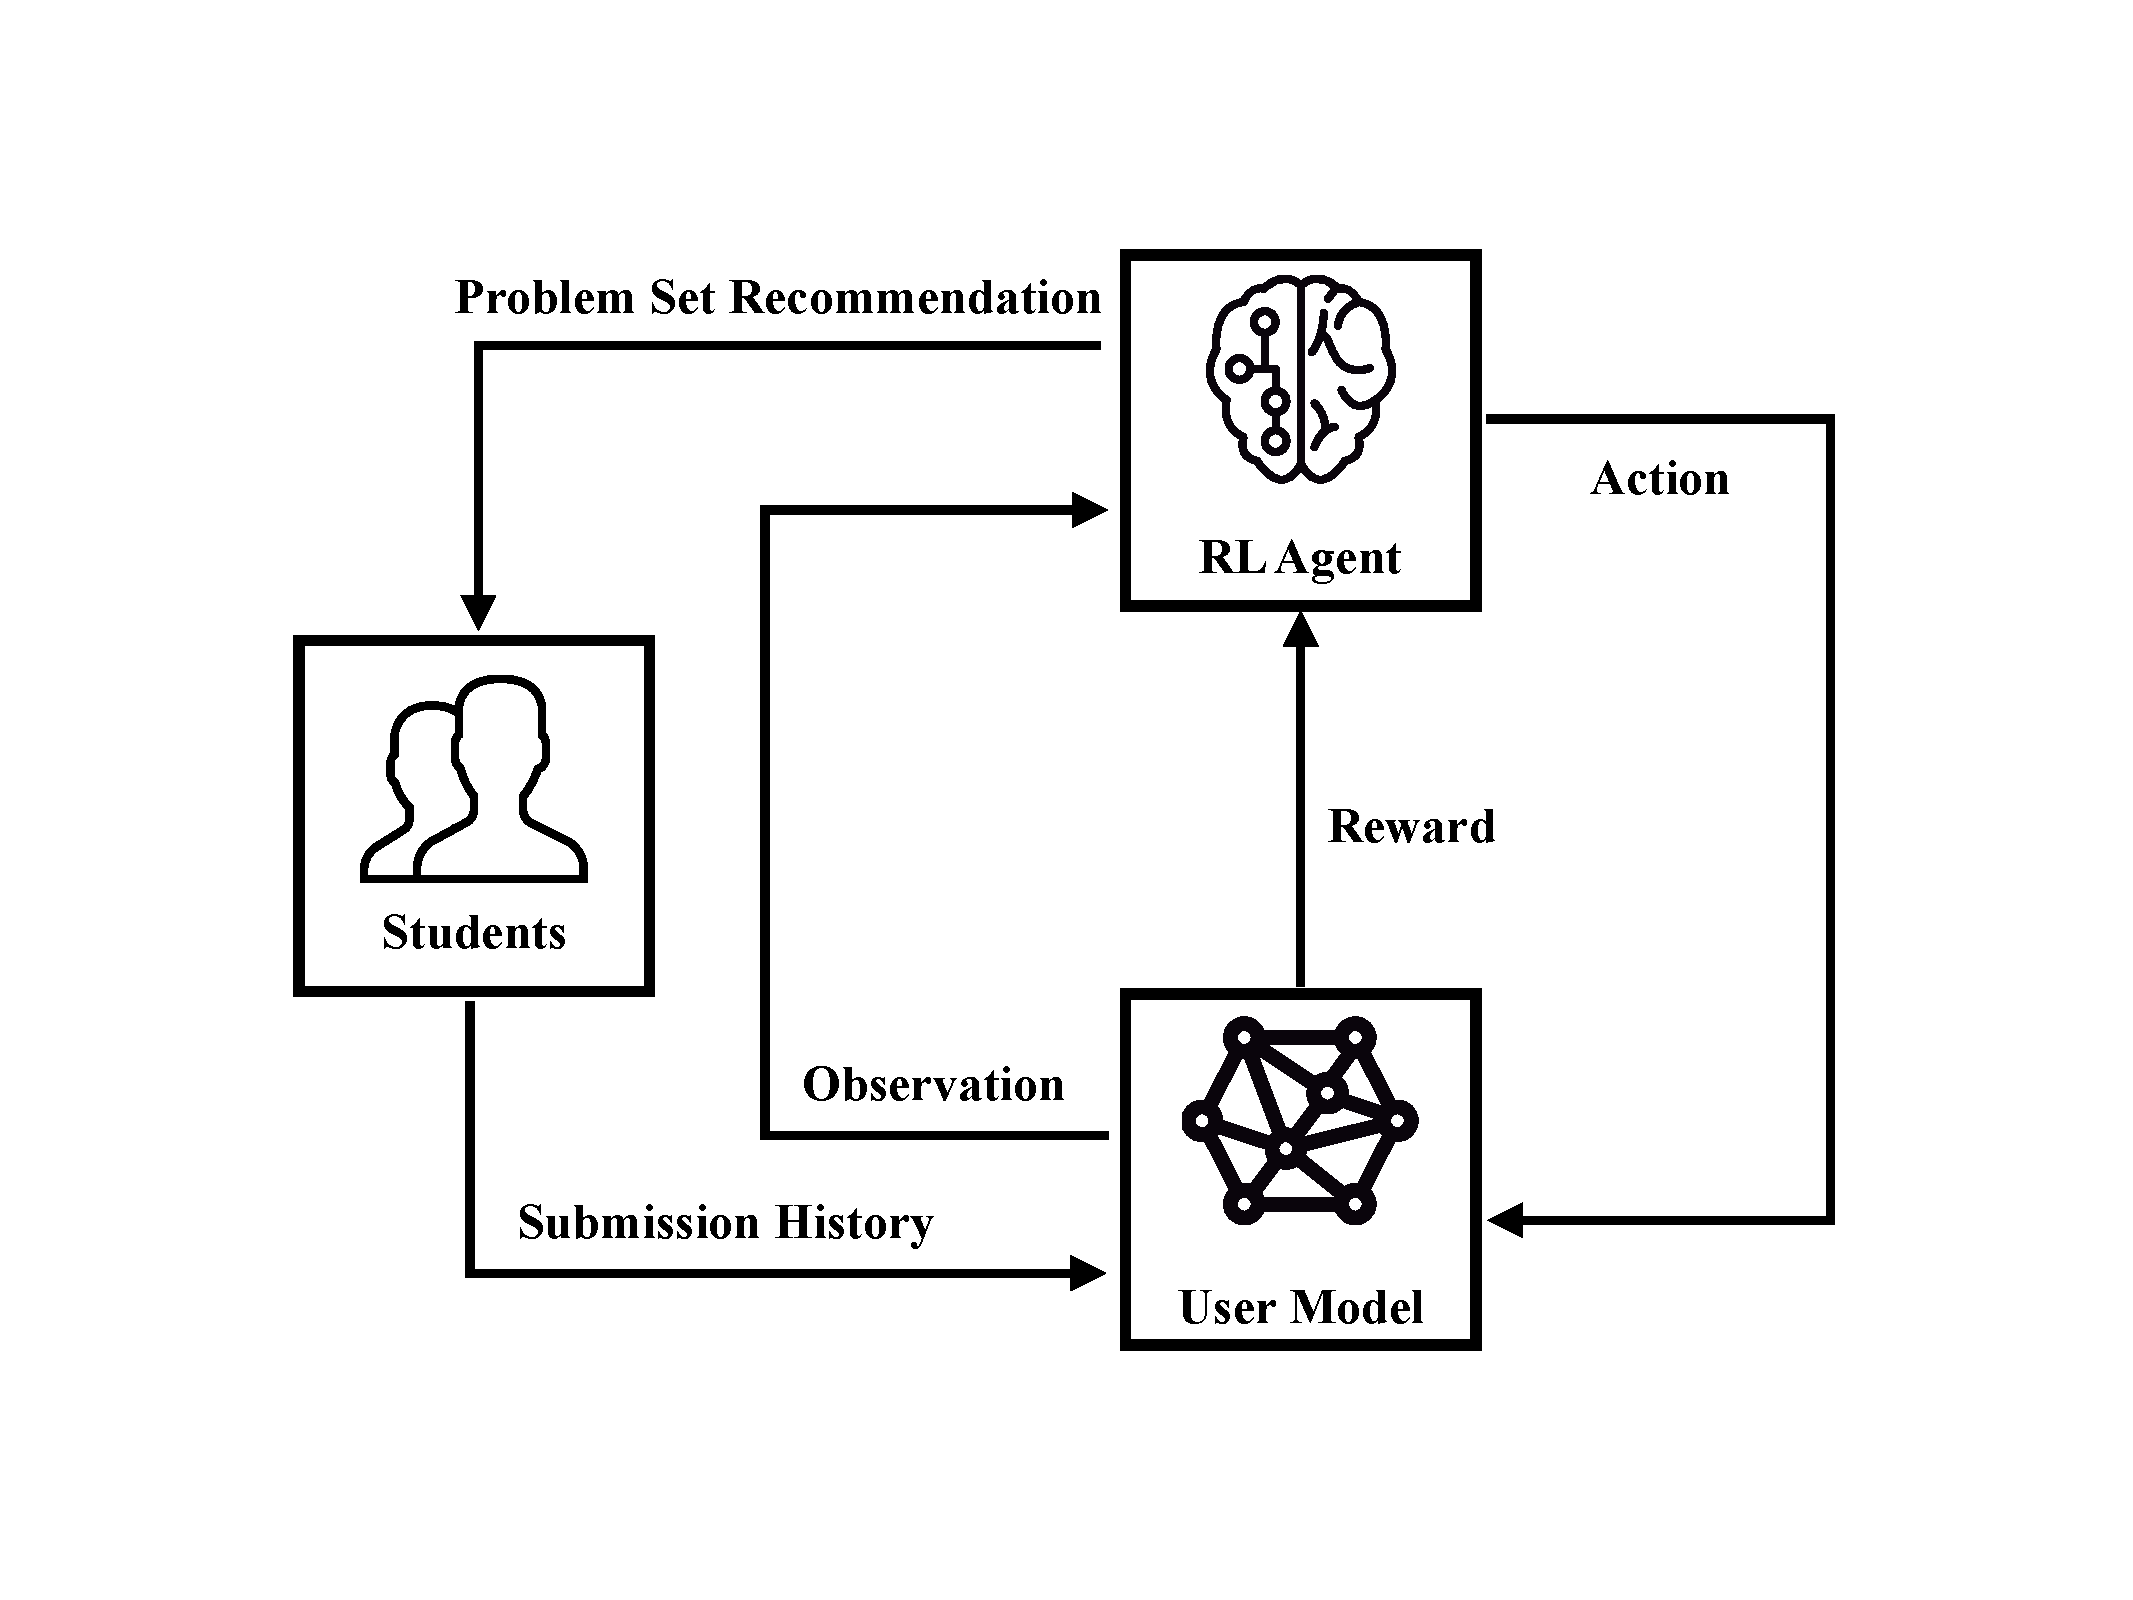
\includegraphics[width=0.62\textwidth]{img/system-design.pdf}
        \caption{System Design}
        \label{fig:system-design}
    \end{figure}

    Therefore, we developed another approach.
    Figure \ref{fig:system-design} shows the design of our work.
    We firstly trained a \emph{user model} to capture students' mindsets using the existing submission records.
    Then, we programmed the reinforcement learning to interact with the user model.
    This real-time interaction enabled the successful training process.
    And this reinforcement learning agent can in turn design problem sets for students.



















